\section{Auswertung}
	\label{sec:auswertung}

	\subsection{Filterkurve des Selektivverst"arkers} % (fold)
	\label{sub:subsection_name}
	
	Die Untersuchung der Filterkurve des Selektiv-Verst"arkers ergab die in Tabelle \ref{tabelle:aufgabe_a} aufgelisteten Werte.
	Daraus ergibt sich der Graph \ref{graph:aufgabe_a}.
	Aus diesem lassen sich die Werte f"ur $\nu_\mathrm{0}$, $\nu_\mathrm{+}$ und $\nu_\mathrm{-}$ ablesen:

	\begin{eqnarray*}
		\nu_\mathrm{0} &=& \SI{34.9}{\kilo\hertz} \, ,\\
		\nu_\mathrm{+} &=& \SI{35.10 (2)}{\kilo\hertz} \, ,\\
		\nu_\mathrm{-} &=& \SI{34.72 (2)}{\kilo\hertz} \, .
	\end{eqnarray*}

	Aus diesen l"asst sich die G"ute mithilfe von Gleichung \eqref{Gleichung:Guete} berechnen.

	\begin{equation*}
		Q = \SI{91.84 (684)}{}
	\end{equation*}

	Der Fehler ergibt sich mittels Gau"s'scher Fehlerfortpflanzung:

	\begin{eqnarray*}
		|\frac{\partial Q}{\partial\nu_\mathrm{+}}| &=& |\frac{\partial Q}{\partial\nu_\mathrm{-}}| \, ,\\
		\Delta \nu_\mathrm{+} &=& \Delta \nu_\mathrm{-} \, ,\\
		\Delta Q &=&  \sqrt{2} \cdot \left( |\frac{\partial Q}{\partial\nu_\text{+,-}}| \Delta \nu_\text{+,-} \right) \, .
	\end{eqnarray*}

	Damit weicht die errechnete G"ute Q = $\SI{91.84 (684)}{}$ um etwa $\SI{8.8}{\%}$ von der eingestellten G"ute Q = $100$ ab.

	\begin{table}[!h]
\begin{center}
\begin{tabular}{|r|r|r|r|}
\hline
f[$\SI{}{\kilo\hertz}$] & U[$\SI{}{\milli\volt}$] & f[$\SI{}{\kilo\hertz}$] & U[$\SI{}{\milli\volt}$]\\
\hline
\hline
25.0 &	0.0 &	35.1 &	6.1 \\	
30.0 &	0.2 &	35.2 &	4.9 \\	
30.5 &	0.2 &	35.3 &	4.0 \\	
31.0 &	0.3 &	35.4 &	3.4 \\	
31.5 &	0.4 &	35.5 &	2.9 \\	
32.0 &	0.5 &	35.6 &	2.5 \\	
32.5 &	0.6 &	35.7 &	2.2 \\	
33.0 &	0.7 &	35.8 &	2.0 \\	
33.5 &	1.1 &	35.9 &	1.8 \\	
34.0 &	1.8 &	36.0 &	1.6 \\	
34.1 &	2.0 &	36.5 &	1.1 \\	
34.2 &	2.3 &	37.0 &	0.8 \\	
34.3 &	2.7 &	37.5 &	0.6 \\	
34.4 &	3.1 &	38.0 &	0.5 \\	
34.5 &	3.8 &	38.5 &	0.4 \\	
34.6 &	4.6 &	39.0 &	0.3 \\	
34.7 &	5.9 &	39.5 &	0.3 \\	
34.8 &	7.4 &	40.0 &	0.2 \\	
34.9 &	8.6 &	40.5 &	0.0 \\	
35.0 &	7.4 &  & \\
\hline
\end{tabular}
\end{center}

	\begin{figure}[!h]
		\centering
		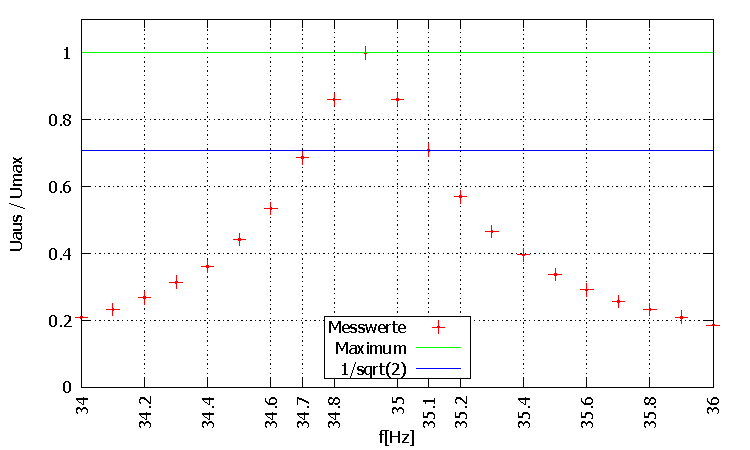
\includegraphics[width = 14cm]{img/arschlecken.pdf}
		\caption{Filterkurve des Selektivverst"arkers}
		\label{graph:aufgabe_a}
	\end{figure}

	\clearpage


	\subsection{Bestimmung der Suszeptibilit"at} % (fold)
	\label{sub:bestimmung_der_suszeptibilit_t}

	F"ur die Messung der Suszeptibilit"at wird eine Spule mit den Eigenschaften:

	\begin{eqnarray*}
		n &=& 250 \,\\
		F &=& \SI{0.866}{\centi\meter^2} \, ,\\
		L &=& \SI{13.5}{\centi\meter} \, , \\
		R &=& \SI{0.7}{\ohm} \, ,
	\end{eqnarray*}

	verwendet.

	Bei der Messung zur Bestimmung der Suszeptibilit"at ergaben sich die Werte in den Tabellen \ref{tabelle:aufgabe_b_Dy}, \ref{tabelle:aufgabe_b_Nd} und \ref{tabelle:aufgabe_b_Gd}.

	Die Mittelwerte sind in Tabelle \ref{Mittelwerte} aufgef"uhrt.

	Bei der Bestimmung der Suszeptibilit"at mit den Gleichungen \eqref{curie}, \eqref{chi_u} und \eqref{chi_r} wurden zus"atzlich die  Werte aus den Tabellen \ref{daten} und \ref{massen} verwendet.

	$A_\mathrm{real}$ ergiebt sich mithilfe der Gleichung:

	\begin{equation}
		A_\mathrm{real} = \frac{M}{L \rho} \, .
	\end{equation}

	Die Verst"arkung durch den Linear- und Selektivverst"arker ergab eine Verst"arkung um einen Faktor von $86.73$.

	F"ur die Berechnung der Suszeptibilit"at nach Gleichung \eqref{curie} wurden die vorgegebenen Werte Verwendet:

	\begin{eqnarray*}
		S &=& \frac{5}{2} \, ,\\
		L &=& 6 \, ,\\
		J &=& \frac{9}{2} \, .
	\end{eqnarray*}

	F"ur die Temperatur wurden $T = \SI{295}{\kelvin}$ benutzt und f"ur die Anzahl der Momente pro Volumen $N$ die Werte aus Tabelle \ref{massen}.

	Bei der Berechnung nach Gleichung \eqref{chi_u} wird f"ur $A$ der $A_\mathrm{real}$ Wert benutzt. Die $\SI{1}{\volt}$ Eingangsspannung wird durch die Verst"arker auf $U_\mathrm{sp} = \SI{86.73}{\volt}$ verst"arkt.
	$U_\mathrm{br}$ wird aus Tabelle \ref{Mittelwerte} benutzt.

	F"ur die dritte Methode nach Gl. \eqref{chi_r} wird auch $A_\mathrm{real}$ benutzt. Der feste Widerstand ist mit $R_\mathrm{3} = \SI{998}{\ohm}$ gegeben.
	$\Delta R$ ergibt sich aus Tabelle \ref{Mittelwerte}.

	Die Ergebnisse sind in Tabelle \ref{suszep} angegeben.

	
\begin{table}[!h]
\begin{center}
\begin{tabular}{|l|r|r|r|r|r|}
\hline
 &&&&&\\
 Probe & $\chi_\mathrm{exp1}$ Widerstand & $\chi_\mathrm{exp2}$ Spannung & $\chi_\mathrm{theo}$ & $\Delta \chi_\mathrm{1}$ & $\Delta \chi_\mathrm{2}$ \\
\hline
\hline

Dysprosium & $\SI{0.0239 (14)}{}$ & $\SI{0.0234 (1)}{}$ & $\SI{0.0253}{}$ & $\SI{5.86}{\%}$ & $\SI{8.12}{\%}$\\
Neodym     & $\SI{0.0026 (21)}{}$ & $\SI{0.0010 (1)}{}$ & $\SI{0.0030}{}$ & $\SI{15.38}{\%}$ & $\SI{200}{\%}$ \\
Gadolinium & $\SI{0.0110 (14)}{}$ & $\SI{0.0101 (1)}{}$ & $\SI{0.0137}{}$ & $\SI{24.55}{\%}$ & $\SI{35.64}{\%}$\\

\hline
\end{tabular}
\caption{Werte f"ur die Suszeptibilit"at mit 3 verschiedenen Messtechniken. $\chi_\mathrm{exp1}$ nach Gl. \eqref{chi_r}, $\chi_\mathrm{exp2}$ nach Gl. \eqref{chi_u} und $\chi_\mathrm{theo}$ nach Gl. \eqref{curie}}
\label{suszep}
\end{center}
\end{table}
	
\begin{table}[!h]
\begin{center}
\begin{tabular}{|l|r|r|r|r|}
\hline
 & &&&\\
Probe & Masse\,[$\SI{}{\gram}$] & L"ange\,[$\SI{}{\centi\meter}$] & Dichte\,[$\SI{}{\gram\per\centi\meter^3}$] & $A_\mathrm{real}$\,[$\SI{}{\centi\meter^2}$]\\
\hline
\hline

Dysprosium & 16.6 & 17.7 & 7800 & 0.12\\
Neodym     & 9.0  & 16.3 & 7240 & 0.08\\
Gadolinium & 14.8 & 16.6 & 7400 & 0.12\\

\hline
\end{tabular}
\caption{Daten der Messproben.}
\label{daten}
\end{center}
\end{table}
	
\begin{table}[!h]
\begin{center}
\begin{tabular}{|l|r|r|r|r|r|r|}
\hline
 & & & & & & \\
Probe & $\bar R_\mathrm{0}$\,[$\SI{}{\milli\ohm}$]& $\Delta R_\mathrm{0}$\,[$\SI{}{\milli\ohm}$] & $\bar U_\mathrm{0}$\,[$\SI{}{\milli\volt}$] & $\Delta U_\mathrm{0}$\,[$\SI{}{\milli\volt}$] & $\bar U_\mathrm{1}$\,[$\SI{}{\milli\volt}$] & $\Delta U_\mathrm{1}$\,[$\SI{}{\milli\volt}$]\\
\hline
\hline

Dysprosium & 2872 & 7.85 & 4.02 & 0.06 & 74.40 & 0.40\\
Neodym & 2832 & 12.30 & 3.90 & 0.03 & 5.88 & 0.24\\
Gadolinium & 2839 & 8.70 & 3.86 & 0.02 & 34.20 & 0.37\\

\hline
\end{tabular}
\end{center}
\begin{center}
\begin{tabular}{|r|r|r|r|}
\hline
&&&\\
$\bar R_\mathrm{1}$\,[$\SI{}{\milli\ohm}$] & $\Delta R_\mathrm{1}$\,[$\SI{}{\milli\ohm}$] & $\overline{\Delta R}$\,[$\SI{}{\milli\ohm}$] & $\Delta(\Delta R)$\,[$\SI{}{\milli\ohm}$]\\
\hline
\hline
1220 & 6.30 & 1652 & 10.55\\
2719 & 7.50 & 118  & 6.80\\
2075 & 10.85 & 764 & 9.65\\
\hline
\end{tabular}
\caption\,{Mittelwerte und Standardabweichung der Probenwerte.}
\label{Mittelwerte}
\end{center}
\end{table}
	
\begin{table}[!h]
\begin{center}
\begin{tabular}{|l|r|r|r|r|}
\hline
&&&&\\
Probe & $\rho$[$\SI{}{\kilo\gram\per\meter^3}$] & M[$\SI{}{\kilo\gram/\mol}$] & M[$\SI{}{\kilo\gram}$] & N[$\SI{}{1\per\meter^3}$]\\
\hline
\hline

	$Dy_2O_3$ & 7800 & 0.3730 & $\SI{6.19 e-25}{}$ & $\SI{2.52 e28}{}$\\
	$Nd_2O_3$ & 7240 & 0.3365 & $\SI{5.59 e-25}{}$ & $\SI{2.59 e28}{}$\\
	$Gd_2O_3$ & 7400 & 0.3625 & $\SI{6.02 e-25}{}$ & $\SI{2.46 e28}{}$\\

\hline
\end{tabular}
\caption{Massen der Messproben.}
\label{massen}
\end{center}
\end{table}
	\begin{table}[!h]
\begin{center}
\begin{tabular}{|r|r|r|r|r|r|r|}
\hline
&&&&&&\\
$R_\mathrm{0}$\,[$\SI{}{\milli\ohm}$] & $U_\mathrm{0}$\,[$\SI{}{\milli\volt}$] & $\Delta U_\mathrm{0}$\,[$\SI{}{\milli\volt}$] & $U_\mathrm{1}$\,[$\SI{}{\milli\volt}$] & $\Delta U_\mathrm{1}$\,[$\SI{}{\milli\volt}$] & $R_\mathrm{1}$\,[$\SI{}{\milli\ohm}$] & $\Delta R$\,[$\SI{}{\milli\ohm}$]\\
\hline
\hline

2850 & 3.9 & 0.1 & 73 & 1 & 1210 & 1640\\
2865 & 3.9 & 0.1 & 75 & 1 & 1230 & 1635\\
2890 & 4.1 & 0.1 & 75 & 1 & 1230 & 1660\\
2865 & 4.0 & 0.1 & 74 & 1 & 1230 & 1635\\
2890 & 4.2 & 0.1 & 75 & 1 & 1200 & 1690\\

\hline
\end{tabular}
\caption[Messwerte zu Aufgabenteil b]{Gemessene Werte zur Bestimmung der Suszeptibilit"at von Dysprosium.}
\label{tabelle:aufgabe_b_Dy}
\end{center}
\end{table}
	\begin{table}[!h]
\begin{center}
\begin{tabular}{|r|r|r|r|r|r|r|}
\hline
R0[$\SI{}{\ohm}$] & U0[$\SI{}{\milli\volt}$] & $\Delta$U0[$\SI{}{\milli\volt}$] & U1[$\SI{}{\milli\volt}$] & $\Delta$U1[$\SI{}{\milli\volt}$] & R1[$\SI{}{\ohm}$] & $\Delta$R[$\SI{}{\ohm}$]\\
\hline
\hline

570 & 4.0 & 0.1 & 6.5 & 0.1 & 543 & 27\\
557 & 3.9 & 0.1 & 5.3 & 0.1 & 537 & 20\\
570 & 3.9 & 0.1 & 6.4 & 0.1 & 544 & 26\\
569 & 3.9 & 0.1 & 5.5 & 0.1 & 545 & 24\\
566 & 3.8 & 0.1 & 5.7 & 0.1 & 545 & 21\\

\hline
\end{tabular}
\caption[Messwerte zu Aufgabenteil b]{Gemessene Werte zur Bestimmung der Suszeptibilit"at von Neodym}
\label{tabelle:aufgabe_b_Nd}
\end{center}
\end{table}
	
\begin{table}[!h]
\begin{center}
\begin{tabular}{|r|r|r|r|r|r|r|}
\hline
R0[$\SI{}{\ohm}$] & U0[$\SI{}{\milli\volt}$] & $\Delta$U0[$\SI{}{\milli\volt}$] & U1[$\SI{}{\milli\volt}$] & $\Delta$U1[$\SI{}{\milli\volt}$] & R1[$\SI{}{\ohm}$] & $\Delta$R[$\SI{}{\ohm}$]\\
\hline
\hline

568 & 3.8 &	0.1 & 35 & 1 & 410 & 158 \\
568 & 3.9 &	0.1 & 34 & 1 & 417 & 151 \\
562 & 3.9 &	0.1 & 34 & 1 & 410 & 152 \\
568 & 3.8 &	0.1 & 33 & 1 & 421 & 147 \\
573 & 3.9 &	0.1 & 35 & 1 & 417 & 156 \\

\hline
\end{tabular}
\caption[Messwerte zu Aufgabenteil b]{Gemessene Werte zur Bestimmung der Suszeptibilit"at von Gadolinium}
\label{tabelle:aufgabe_b_Gd}
\end{center}
\end{table}

	\clearpage